\documentclass[aspectratio=169, table, 12pt]{beamer}

% Preamble bersama seluruh slide mata kuliah ini.
% Dipanggil dari slides/sessionXX/sessionXX.tex tepat sesudah baris
% \documentclass[aspectratio=169, table, 12pt]{beamer}
% Paket tambahan yang hanya dibutuhkan satu sesi ditulis di berkas sesi itu.

\usepackage{colortbl}
\usepackage{xcolor}
\usepackage{listings}
\usepackage{tabularx}
\usepackage{booktabs}
\usepackage{tikz}
\usepackage{pgfplots}
\pgfplotsset{compat=1.18}
\usetikzlibrary{arrows.meta, positioning, calc, fit, shapes.geometric,
	shapes.multipart, backgrounds, matrix, chains, trees}

\makeatletter
\def\input@path{{../theme/}}
\makeatother
\graphicspath{{../theme/}{../../figures/}}
\usetheme{Pradita}

\definecolor{praditagreen}{RGB}{37, 113, 71}

% Tema membuat garis tabel berwarna putih. Dikembalikan agar tabel terbaca.
\arrayrulecolor{black}
\setlength{\arrayrulewidth}{0.5pt}

\lstdefinelanguage{yaml}{
	basicstyle=\ttfamily\scriptsize,
	keywordstyle=\color{blue}\bfseries,
	commentstyle=\color{gray}\itshape,
	stringstyle=\color{red},
	showstringspaces=false,
	breaklines=true,
	frame=lines,
	numbers=none,
	backgroundcolor=\color{lightgray!10},
	tabsize=2,
	morecomment=[l]{\#}
}

\lstdefinelanguage{json}{
	basicstyle=\ttfamily\scriptsize,
	stringstyle=\color{red},
	commentstyle=\color{gray},
	breaklines=true,
	showstringspaces=false,
	tabsize=2,
	numbers=none,
	frame=lines,
	backgroundcolor=\color{lightgray!10},
	string=[s]{"}{"}
}

\lstdefinelanguage{bash}{
	keywords={},
	basicstyle=\ttfamily\scriptsize,
	ndkeywords={docker, kubectl, helm, curl, git, terraform},
	ndkeywordstyle=\color{purple}\bfseries,
	sensitive=true,
	commentstyle=\color{gray},
	numbers=none,
	breaklines=true,
	frame=lines,
	backgroundcolor=\color{lightgray!10},
	tabsize=2,
	comment=[l]{\#},
	showstringspaces=false
}

\lstdefinelanguage{http}{
	keywords={GET, POST, PUT, PATCH, DELETE, HEAD, OPTIONS, HTTP},
	basicstyle=\ttfamily\scriptsize,
	keywordstyle=\color{blue}\bfseries,
	sensitive=true,
	numbers=none,
	breaklines=true,
	frame=lines,
	backgroundcolor=\color{lightgray!10},
	tabsize=2,
	showstringspaces=false
}

\subtitle{IT40713 · Cloud-Native \& Microservices Architecture}
\author{\textbf{Alfa Yohannis}}


\title{\Huge Ekonomi Cloud,\\ \vspace{10pt} FinOps \& Keberlanjutan}

\begin{document}

\frame{\titlepage}

\begin{frame}
  \frametitle{Isi Pertemuan}
  \vspace{14pt}
  \begin{columns}[t]
    \column{0.5\textwidth}
    {\small\tableofcontents[sections={1-4}]}

    \column{0.5\textwidth}
    {\small\tableofcontents[sections={5-8}]}
  \end{columns}
\end{frame}

\begin{frame}{\hfill}
  \centering
  \Huge{\textbf{Mengapa tagihan \textit{cloud}\\bisa naik walaupun\\pasien tidak bertambah?}}
\end{frame}

\section{Tujuan dan Konteks}

\begin{frame}{\hfill}
  \centering
  \Huge{\textbf{Tujuan dan Konteks}}
\end{frame}

\begin{frame}{{\Large Tujuan Pembelajaran}}
  \vspace{10pt}
  \begin{itemize}
    \item Membandingkan struktur biaya pusat data sendiri dan \textit{cloud}
          dengan pendekatan TCO.
    \item Menjelaskan prinsip, fase, dan peran dalam FinOps Framework 2026.
    \item Merumuskan metrik biaya per unit dan metrik jejak karbon untuk satu
          layanan.
  \end{itemize}
\end{frame}

\begin{frame}{{\Large Diagram Konsep Bab 3}}
  \centering
  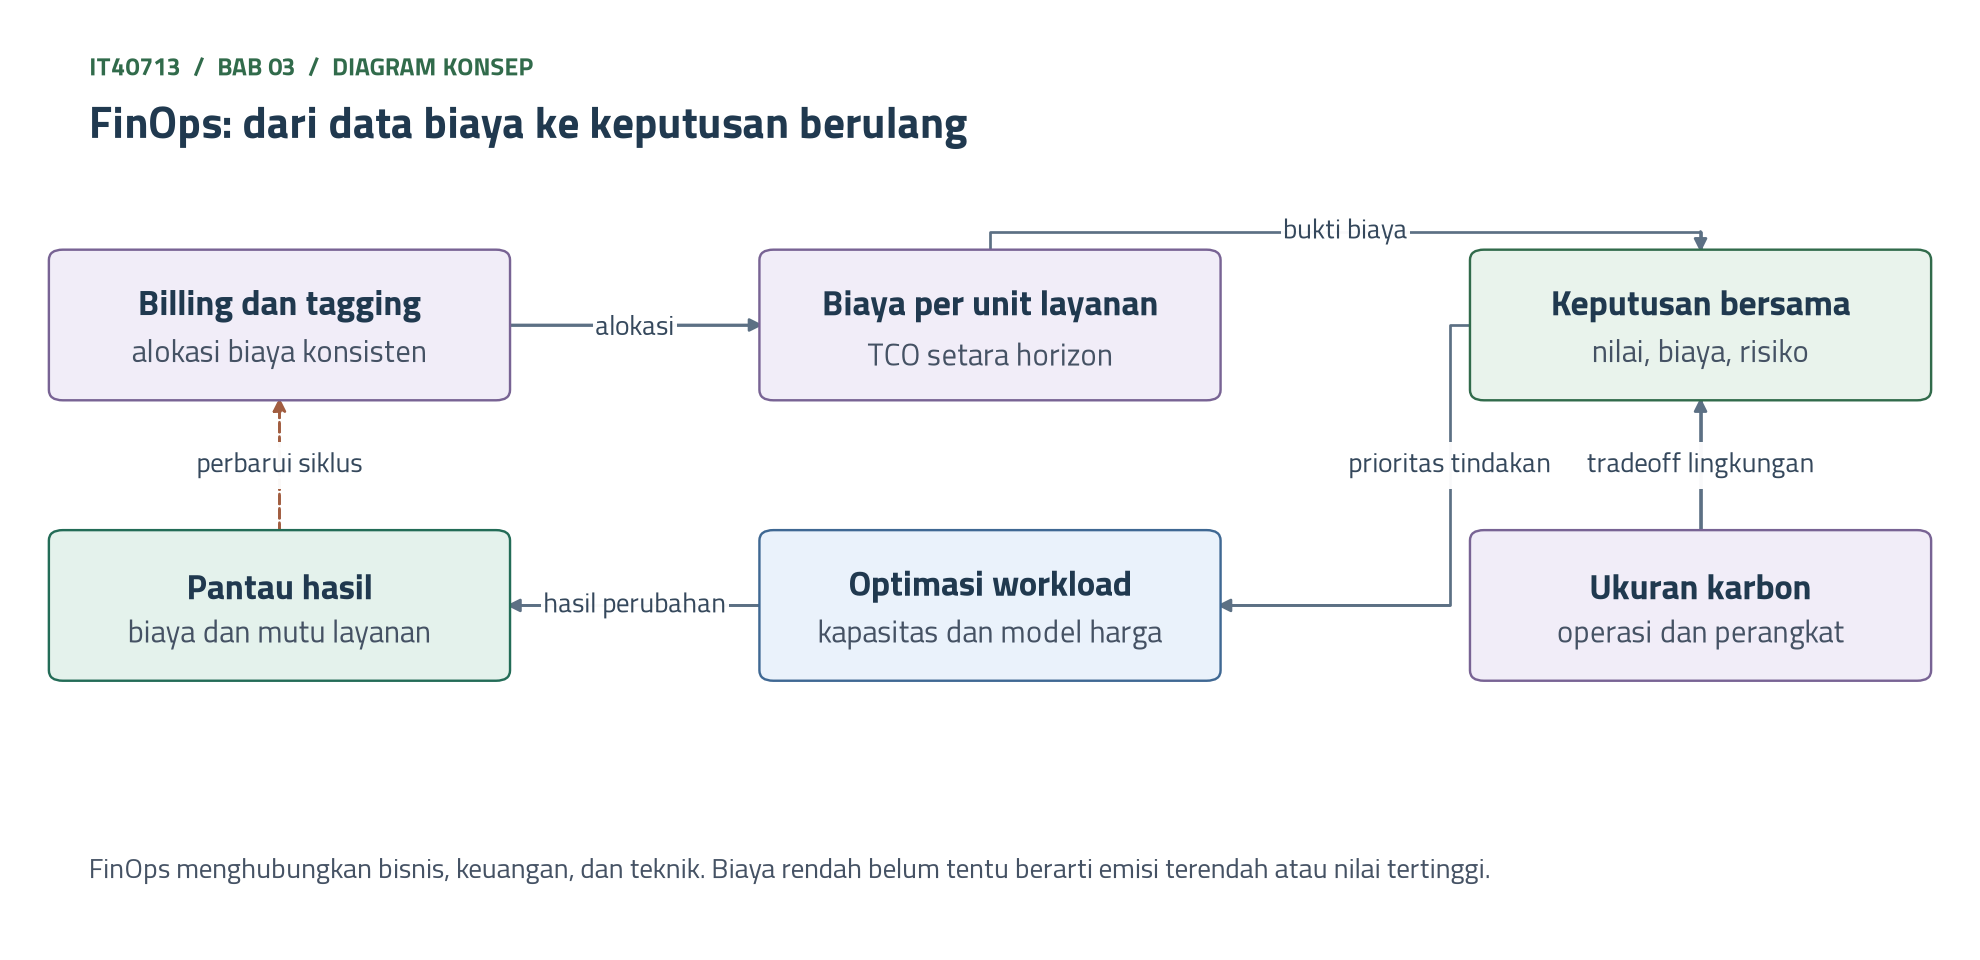
\includegraphics[width=0.96\textwidth,height=0.77\textheight,keepaspectratio]{../../figures/ch03-diagram-konsep.png}
\end{frame}

\section{CapEx, OpEx, dan TCO}

\begin{frame}{\hfill}
  \centering
  \Huge{\textbf{CapEx, OpEx, dan TCO}}
\end{frame}

\begin{frame}{{\Large CapEx dan OpEx}}
  \footnotesize
  \begin{tabularx}{\textwidth}{>{\raggedright\arraybackslash}p{2.6cm}
      >{\raggedright\arraybackslash}X >{\raggedright\arraybackslash}X}
    \hline
    \textbf{Aspek} & \textbf{CapEx (pusat data sendiri)} & \textbf{OpEx (\textit{cloud})} \\
    \hline
    Pencatatan & Aset di neraca, disusutkan & Beban di laba rugi bulan itu \\
    \hline
    Arus kas & Besar di awal, lalu stabil & Kecil di awal, naik turun \\
    \hline
    Saat keputusan & Sekali, siklus anggaran modal & Setiap kali sumber daya
      dibuat \\
    \hline
    Risiko utama & Kapasitas menganggur & Tagihan membengkak \\
    \hline
  \end{tabularx}

  \vspace{10pt}
  \small
  Analogi: membeli mobil operasional atau memakai taksi daring. Pilihan
  ditentukan pola pemakaian, bukan mana yang terdengar lebih modern.
\end{frame}

\begin{frame}{{\Large Dua Contoh dari Medikara Health}}
  \vspace{10pt}
  \begin{itemize}
    \item Server SIMRS rumah sakit Bekasi Rp2,4 miliar, disusutkan lima tahun:
          Rp480 juta per tahun.
    \item Server itu dibeli untuk puncak pagi, padahal pemanfaatan prosesor
          rata-rata sekitar 25 persen.
    \item Medikara+ di \textit{cloud}: Rp57 juta pada bulan biasa, Rp79,3 juta
          pada bulan kampanye vaksinasi.
    \item Tidak ada aset dibeli, tetapi selisih Rp22,3 juta harus dijelaskan
          kepada direksi.
  \end{itemize}
\end{frame}

\begin{frame}{{\Large TCO sebagai Gunung Es}}
  \centering
  \eadiagram{../../figures/ch03-gunung-es-tco.tex}
\end{frame}

\begin{frame}{{\Large Perbandingan TCO yang Jujur}}
  \vspace{10pt}
  \begin{itemize}
    \item Masa sama, misalnya lima tahun untuk kedua sisi.
    \item Lingkup sama: bila \textit{cloud} memasukkan DR, pusat data sendiri
          juga.
    \item Tingkat layanan setara: ketersediaan dan frekuensi cadangan.
    \item Tenaga kerja dan pelatihan ikut dihitung.
    \item Asumsi ditulis dan diuji kepekaannya.
  \end{itemize}
  \vspace{6pt}
  {\small TCO menjawab "berapa biayanya"; \textit{business case} menjawab
  "apakah sepadan" (rinci di IT40513).}
\end{frame}

\begin{frame}{{\Large Kasus Medikara: TCO Kasar SIMRS Bekasi}}
  \scriptsize
  \begin{tabularx}{\textwidth}{>{\raggedright\arraybackslash}X r r r}
    \hline
    \textbf{Komponen (juta rupiah, lima tahun)} & \textbf{Sendiri}
      & \textbf{Opsi A} & \textbf{Opsi B} \\
    \hline
    Perangkat keras; ruang, listrik, pendingin & 2.850 & 0 & 0 \\
    \hline
    Sumber daya \textit{cloud} & 0 & 3.300 & 2.040 \\
    \hline
    Lisensi & 750 & 750 & 750 \\
    \hline
    Tenaga kerja & 1.800 & 900 & 900 \\
    \hline
    Cadangan, DR, jaringan, transfer data keluar & 500 & 550 & 550 \\
    \hline
    Migrasi, operasi paralel, pelatihan & 0 & 510 & 510 \\
    \hline
    \textbf{Total lima tahun} & \textbf{5.900} & \textbf{6.010} & \textbf{4.750} \\
    \hline
    Biaya per kunjungan pasien (rupiah) & 5.619 & 5.724 & 4.524 \\
    \hline
  \end{tabularx}

  \vspace{8pt}
  \small
  Opsi A (\textit{rehost} \textit{on-demand}) Rp110 juta lebih mahal. Opsi B
  (\textit{rightsizing} dan komitmen) hemat Rp1,15 miliar, sekitar 19,5 persen.
\end{frame}

\section{Model Harga Cloud}

\begin{frame}{\hfill}
  \centering
  \Huge{\textbf{Model Harga Cloud}}
\end{frame}

\begin{frame}{{\Large Tiga Cara Membayar Kapasitas yang Sama}}
  \vspace{10pt}
  \begin{itemize}
    \item \textit{On-demand}: per detik atau per jam, tanpa janji, paling mahal
          per unit.
    \item Komitmen satu atau tiga tahun: AWS menyebut potongan Savings Plans
          sampai 72 persen.
    \item \textit{Spot}: kapasitas menganggur, sampai 90 persen lebih murah,
          bisa ditarik dengan pemberitahuan dua menit.
    \item Angka 72 dan 90 persen adalah batas atas, bukan jaminan.
    \item Analogi: parkir harian, langganan bulanan, dan lahan kosong tetangga.
  \end{itemize}
\end{frame}

\begin{frame}{{\Large Pola Beban Menentukan Model Harga}}
  \centering
  \eadiagram{../../figures/ch03-pola-beban-harga.tex}

  \vspace{4pt}
  {\small Beban dasar SIMRS: komitmen. Lonjakan Medikara+: \textit{on-demand}.
  Pengolahan laboratorium malam: \textit{spot}.}
\end{frame}

\begin{frame}{{\Large Risiko Komitmen Berlebih}}
  \vspace{6pt}
  \[
    \text{pemanfaatan impas} = 1 - \text{potongan komitmen}
  \]
  \begin{itemize}
    \item Potongan 40 persen: impas pada pemanfaatan 60 persen.
    \item Komitmen 100 unit, Rp600 per unit-jam, 730 jam: Rp43,8 juta per bulan.
    \item Pemakaian 70 unit: hemat Rp7,3 juta. Pemakaian 50 unit: rugi
          Rp7,3 juta.
    \item Urutan aman: \textit{rightsizing}, komit pada lantai beban, tambah
          bertahap, pantau bulanan.
  \end{itemize}
\end{frame}

\section{FinOps Framework 2026}

\begin{frame}{\hfill}
  \centering
  \Huge{\textbf{FinOps Framework 2026}}
\end{frame}

\begin{frame}{{\Large Apa Itu FinOps}}
  \vspace{10pt}
  \begin{itemize}
    \item Kerangka operasional dan praktik budaya yang memaksimalkan nilai
          bisnis teknologi.
    \item Keputusan berbasis data yang cepat dan akuntabilitas lewat
          kolaborasi teknik, keuangan, dan bisnis.
    \item Tujuannya nilai, bukan tagihan sekecil mungkin.
    \item Analogi: keluarga besar dengan satu meteran listrik, lalu meteran
          per rumah dan rapat bulanan.
  \end{itemize}
\end{frame}

\begin{frame}{{\Large Enam Prinsip FinOps}}
  \footnotesize
  \begin{tabularx}{\textwidth}{>{\raggedright\arraybackslash}p{6.6cm}
      >{\raggedright\arraybackslash}X}
    \hline
    \textbf{Prinsip} & \textbf{Contoh di Medikara} \\
    \hline
    \textit{Teams need to collaborate} & Rapat biaya bulanan lintas fungsi \\
    \hline
    \textit{Business value drives technology decisions} & Biaya naik saat janji
      temu naik dianggap wajar \\
    \hline
    \textit{Everyone takes ownership for their technology usage} & Lingkungan
      uji dimatikan di luar jam kerja \\
    \hline
    \textit{FinOps data should be accessible, timely, and accurate}
      & \textit{Dashboard} biaya harian \\
    \hline
    \textit{FinOps should be enabled centrally} & Analis FinOps mengelola
      komitmen grup \\
    \hline
    \textit{Take advantage of the variable cost model of the cloud} & Kapasitas
      naik saat kampanye vaksinasi \\
    \hline
  \end{tabularx}
\end{frame}

\begin{frame}{{\Large Fase Inform, Optimize, dan Operate}}
  \centering
  \eadiagram{../../figures/ch03-siklus-finops.tex}
\end{frame}

\begin{frame}{{\Large Persona dan Domain}}
  \begin{columns}[t]
    \column{0.46\textwidth}
    \small
    \textbf{Persona inti}
    \begin{itemize}
      \item FinOps Practitioner, Engineering, Finance
      \item Product, Procurement, Leadership
    \end{itemize}
    \textbf{Persona pendukung}
    \begin{itemize}
      \item Aset, keuangan, dan layanan TI
      \item Keamanan dan keberlanjutan
    \end{itemize}

    \column{0.52\textwidth}
    \small
    \textbf{Empat domain}
    \begin{itemize}
      \item Understand Usage \& Cost
      \item Quantify Business Value
      \item Optimize Usage \& Cost
      \item Manage the FinOps Practice, termasuk Executive Strategy Alignment
            (baru 2026)
    \end{itemize}
  \end{columns}
\end{frame}

\begin{frame}{{\Large Scope dan Kategori Teknologi}}
  \vspace{10pt}
  \begin{itemize}
    \item Kategori teknologi: AI, \textit{public cloud}, SaaS, \textit{data
          platform}, \textit{private cloud}, lisensi, pusat data.
    \item \textit{Scope}: batas penerapan FinOps, misalnya per produk, pusat
          biaya, atau lingkungan.
    \item Pusat data ikut dikelola agar perbandingan TCO memakai bahasa yang
          sama.
    \item Kematangan tiap \textit{capability}: \textit{crawl}, \textit{walk},
          \textit{run}.
  \end{itemize}
\end{frame}

\begin{frame}{{\Large Kasus Medikara: Siapa Mengisi Persona Inti}}
  \footnotesize
  \begin{tabularx}{\textwidth}{>{\raggedright\arraybackslash}p{3.4cm}
      >{\raggedright\arraybackslash}X}
    \hline
    \textbf{Persona} & \textbf{Pengisi di Medikara} \\
    \hline
    FinOps Practitioner & Analis FinOps baru di direktorat TI \\
    \hline
    Engineering & Tim infrastruktur pusat dan tim vendor Medikara+ \\
    \hline
    Finance & Bagian akuntansi manajemen dan anggaran \\
    \hline
    Product & Pemilik produk Medikara+, kepala instalasi SIMRS \\
    \hline
    Procurement & Bagian pengadaan, karena komitmen adalah kontrak \\
    \hline
    Leadership & Direktur keuangan, direktur TI, direktur utama \\
    \hline
  \end{tabularx}
\end{frame}

\section{Alokasi dan Unit Economics}

\begin{frame}{\hfill}
  \centering
  \Huge{\textbf{Alokasi dan Unit Economics}}
\end{frame}

\begin{frame}{{\Large Dari Tagihan Mentah ke Biaya per Unit}}
  \centering
  \eadiagram{../../figures/ch03-alur-alokasi.tex}

  \vspace{6pt}
  {\small Lima \textit{tag} wajib: \texttt{layanan}, \texttt{lingkungan},
  \texttt{fasilitas}, \texttt{pusat-biaya}, \texttt{pemilik}. Agustus 2026:
  Rp5 juta dari Rp76,2 juta belum ber-\textit{tag}.}
\end{frame}

\begin{frame}{{\Large Showback dan Chargeback}}
  \footnotesize
  \begin{tabularx}{\textwidth}{>{\raggedright\arraybackslash}p{2.8cm}
      >{\raggedright\arraybackslash}X >{\raggedright\arraybackslash}X}
    \hline
    \textbf{Aspek} & \textbf{\textit{Showback}} & \textbf{\textit{Chargeback}} \\
    \hline
    Yang terjadi & Biaya diperlihatkan & Biaya masuk anggaran unit \\
    \hline
    Syarat data & Cukup akurat untuk dibaca & Akurat, rinci, dan disepakati \\
    \hline
    Dampak & Kesadaran tumbuh tanpa konflik & Unit berhemat, angka bisa
      diperdebatkan \\
    \hline
    Cocok untuk & Tahap awal & Tahap matang \\
    \hline
  \end{tabularx}

  \vspace{10pt}
  \small
  Medikara Health mulai dengan \textit{showback}, karena \textit{tag} belum rapi
  dan cara anggaran rumah sakit hasil akuisisi masih berbeda.
\end{frame}

\begin{frame}{{\Large FOCUS: Satu Skema untuk Banyak Tagihan}}
  \vspace{10pt}
  \begin{itemize}
    \item Spesifikasi terbuka untuk data tagihan, versi 1.4 terbit 2026.
    \item Kolom bersama: \texttt{ServiceCategory}, \texttt{RegionId},
          \texttt{PricingCategory}, \texttt{Tags}.
    \item \texttt{BilledCost}: angka di faktur, dipakai untuk mencocokkan
          tagihan.
    \item \texttt{EffectiveCost}: komitmen disebar ke pemakaian, dipakai untuk
          alokasi.
    \item Komitmen Rp34 juta dengan \texttt{BilledCost} jatuh ke kelompok tanpa
          pemilik.
  \end{itemize}
\end{frame}

\begin{frame}{{\Large Unit Economics: Medikara+}}
  \vspace{6pt}
  \footnotesize
  \begin{tabularx}{\textwidth}{>{\raggedright\arraybackslash}X r r r}
    \hline
    \textbf{Bulan} & \textbf{Biaya \textit{cloud}} & \textbf{Janji temu}
      & \textbf{Per janji temu} \\
    \hline
    Agustus 2026 (biasa) & Rp57 juta & 28.000 & Rp2.036 \\
    \hline
    Oktober 2026 (kampanye vaksinasi) & Rp79,3 juta & 45.000 & Rp1.762 \\
    \hline
  \end{tabularx}

  \vspace{10pt}
  \small
  \begin{itemize}
    \item Tagihan naik 39 persen, biaya per janji temu turun 13 persen.
    \item Unit yang baik: dipahami direksi, data rutin, mengikuti pemicu biaya,
          sulit dimanipulasi.
    \item Sasaran nilai: biaya per kunjungan pasien turun 15 persen dalam dua
          tahun.
  \end{itemize}
\end{frame}

\section{Keberlanjutan dan Jejak Karbon}

\begin{frame}{\hfill}
  \centering
  \Huge{\textbf{Keberlanjutan dan Jejak Karbon}}
\end{frame}

\begin{frame}{{\Large Sumber Emisi dan Pembagian Tanggung Jawab}}
  \vspace{10pt}
  \begin{itemize}
    \item Emisi operasional: listrik server, penyimpanan, jaringan, pendingin.
    \item Emisi melekat: pembuatan, pengiriman, dan pembuangan perangkat.
    \item AWS dan Google Cloud memasukkan keberlanjutan sebagai pilar
          Well-Architected.
    \item Penyedia: efisiensi pusat data. Pelanggan: efisiensi
          \textit{workload}-nya.
    \item Server menganggur di \textit{cloud} tetap membuang energi.
  \end{itemize}
\end{frame}

\begin{frame}{{\Large Software Carbon Intensity (ISO/IEC 21031:2024)}}
  \begin{columns}[c]
    \column{0.42\textwidth}
    \[
      \mathrm{SCI} = \frac{(E \times I) + M}{R}
    \]
    \small
    $E$ energi, $I$ intensitas karbon listrik, $M$ emisi melekat, $R$ satuan
    fungsi.

    \column{0.56\textwidth}
    \scriptsize
    \begin{tabularx}{\linewidth}{>{\raggedright\arraybackslash}X r r}
      \hline
      \textbf{Medikara+ per bulan} & \textbf{Sebelum} & \textbf{Sesudah} \\
      \hline
      $E$ (kWh) & 1.900 & 1.450 \\
      \hline
      $I$ (kg per kWh, asumsi) & 0,70 & 0,70 \\
      \hline
      $M$ (kg) & 300 & 240 \\
      \hline
      $R$ (janji temu) & 28.000 & 28.000 \\
      \hline
      \textbf{SCI (gram per janji temu)} & \textbf{58,2} & \textbf{44,8} \\
      \hline
    \end{tabularx}
  \end{columns}
\end{frame}

\begin{frame}{{\Large Tiga Tuas: Region, Pemanfaatan, Jadwal}}
  \vspace{10pt}
  \begin{itemize}
    \item Region: intensitas karbon berbeda, tetapi rekam medis tetap di
          Indonesia.
    \item Pemanfaatan: satu server 60 persen lebih efisien daripada tiga server
          20 persen.
    \item Jadwal: lingkungan uji dimatikan di luar jam kerja.
    \item Biaya dan karbon umumnya searah, tetapi komitmen besar dan DR bisa
          bertentangan.
    \item Total emisi boleh naik saat layanan tumbuh; SCI yang dijaga turun.
  \end{itemize}
\end{frame}

\section{Aktivitas}

\begin{frame}{{\Large Aktivitas: Model Biaya Awal dan Sasaran Nilai}}
  \small
  \begin{enumerate}
    \item Pilih satu \textit{workload} dari matriks kendala penempatan Bab 2.
    \item Susun biaya kondisi sekarang lima tahun dengan templat TCO.
    \item Perkirakan satu atau dua opsi \textit{cloud}.
    \item Tetapkan satu metrik biaya per unit dan hitung nilai awalnya.
    \item Rumuskan sasaran nilai: angka, arah, batas waktu, metrik pendamping.
  \end{enumerate}
  \vspace{4pt}
  \footnotesize
  Peran: keuangan memimpin struktur biaya; teknis memakai kalkulator harga;
  anggota lain memeriksa asumsi. Berkas: \berkas{sources/chapter03/}.
\end{frame}

\begin{frame}{{\Large Luaran dan Kriteria Penilaian}}
  \footnotesize
  \begin{tabularx}{\textwidth}{>{\raggedright\arraybackslash}X r
      >{\raggedright\arraybackslash}X}
    \hline
    \textbf{Kriteria} & \textbf{Bobot} & \textbf{Bukti yang dicari} \\
    \hline
    Kelengkapan dan kejujuran TCO & 30 persen & Biaya yang sering terlupa ikut
      dihitung \\
    \hline
    Asumsi yang dapat diperiksa & 20 persen & Setiap angka punya sumber \\
    \hline
    Kualitas metrik biaya per unit & 25 persen & Bermakna bagi direksi \\
    \hline
    Sasaran nilai yang terukur & 25 persen & Angka, arah, batas waktu \\
    \hline
  \end{tabularx}

  \vspace{10pt}
  \small
  Luaran C1: templat TCO terisi, lembar sasaran nilai, dan ringkasan satu
  halaman. Data nyata hanya seizin organisasi dan dianonimkan.
\end{frame}

\section{Ringkasan dan Latihan}

\begin{frame}{{\Large Ringkasan}}
  \vspace{10pt}
  \begin{itemize}
    \item \textit{Cloud} mengubah CapEx menjadi OpEx; keputusan biaya pindah ke
          tim teknik.
    \item TCO jujur memasukkan biaya di bawah permukaan; \textit{rehost} apa
          adanya bisa lebih mahal.
    \item Komitmen untuk lantai beban, \textit{on-demand} untuk puncak,
          \textit{spot} untuk \textit{batch}.
    \item FinOps: enam prinsip, tiga fase, persona, domain, dan
          \textit{capability}.
    \item Biaya dan karbon per unit layanan lebih bermakna daripada total
          tagihan.
  \end{itemize}
\end{frame}

\begin{frame}{{\Large Latihan}}
  \vspace{10pt}
  \begin{enumerate}
    \item Jelaskan mengapa tagihan \textit{cloud} sebuah organisasi bisa naik
          walaupun jumlah penggunanya tetap. Berikan tiga penyebab yang mungkin.
    \item Pilih satu layanan Medikara Health dan usulkan metrik biaya per unit
          yang bermakna bagi direksi. Jelaskan alasan pemilihannya.
    \item Kapan model harga berbasis komitmen lebih menguntungkan daripada
          \textit{on-demand}, dan kapan justru merugikan?
  \end{enumerate}
  \vspace{6pt}
  {\small Tabel contoh dan lembar isian ada di naskah Bab 3.}
\end{frame}

\end{document}
